\mysection{Scaling to Real-world Data: KITTI [3]}

%\begin{table}
    % \hfill
    \begin{minipage}[c]{0.3\textwidth}
        \centering
        % \todo[inline]{other results are on their way}
        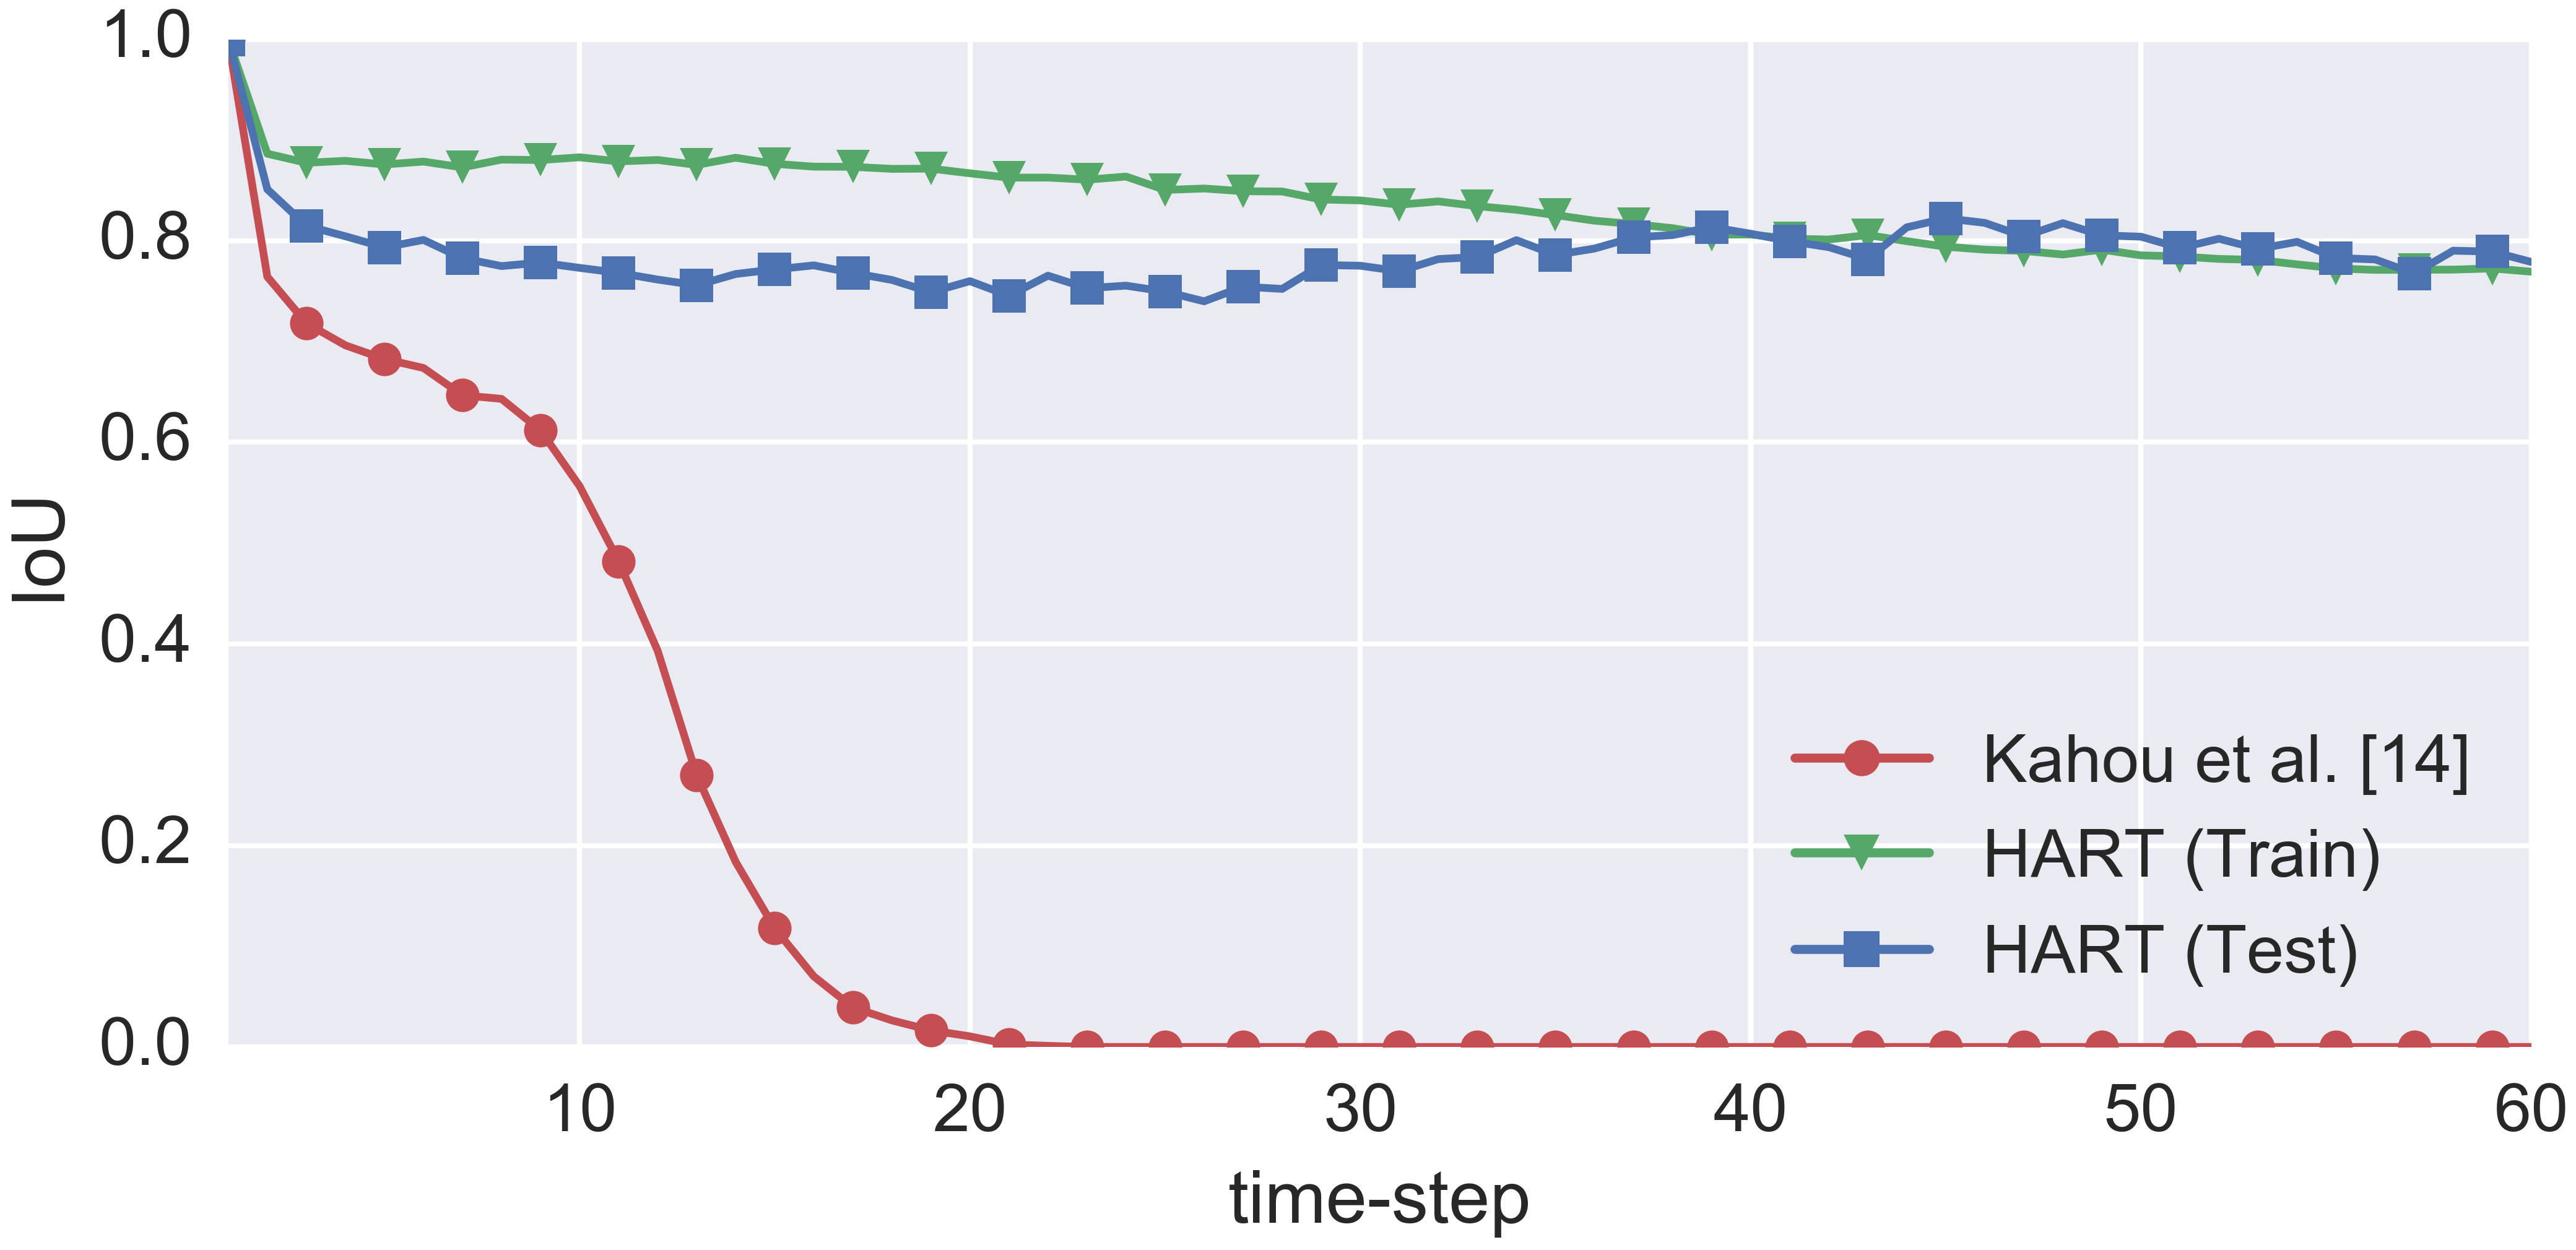
\includegraphics[width=\textwidth]{kitti_iou_fig}
        
        {\large
        \begin{minipage}[c]{0.5\linewidth}
            \centering
            \begin{tabular}{c|c|c|c}
                \multicolumn{4}{c}{Average IoU on KITTI over 60 time-steps}\\
                Kahou \emph{et. al.} [1] & Spatial Att & App Att & HART\\
                \midrule
                0.14 & 0.60 & 0.78 & \B{0.81}
            \end{tabular}
        \end{minipage}
        }\hfill
        \begin{minipage}[c]{0.4\linewidth}
            IoU curves on KITTI over 60 timesteps. HART~(train) presents evaluation on the train set.
        \end{minipage}
    \end{minipage}
    

    \vspace{1em}


%        \begin{tabular}{c|c}
%            \toprule
%            Method                      &   Avg. IoU\\
%            \midrule
%            \citet{Kahou2015ratm}       &   0.14      \\
%            Spatial Att                 &   0.60       \\  
%            % 			Spatial Att with Loss       &   0.70   \\
%            App Att                     &   0.78       \\
%            HART                        &   \B{0.81}   \\
%            \bottomrule
%        \end{tabular}
%        \vspace{1em}
%        Average IoU on KITTI over 60 time-steps.